\section{Ergebnisse und Auswertung}
  
  \subsection{Qualitative Bestimmung von Wasserrückständen und Berechnung chromatographischer Parameter} 
    
    In den folgenden Tabellen befinden sich die Ergebnisse der qualitativen Analyse. 
    
    \begin{table}[H]
      \centering
      \caption[Ergebnisse der qualitativen Analyse (Einzelstandards), Quelle: Autor]{Ergebnisse der qualitativen Analyse (Einzelstandards \SI[mode=text]{50}{ppm}).}
      
      \label{tab:ErgebnisseEinzelstandards}
      \begin{tabular}{@{}l|lllllp{4.5cm}l@{}}
        \toprule
          Peak Nr. & Analyt & $t_0$ in \si{\minute} & $t_R$ in \si{\minute} & $t_N$ in \si{\minute}  & k \\ \midrule
          1 & Carbamazepin & 1.452 & 2.271 & 0.819 & 0.564 \\
          2 & Estradiol & 1.452 & 2.921 & 1.469 & 1.012 \\
          3 & Naproxen & 1.452 & 3.429 & 1.977 & 1.362 \\
          4 & Estron & 1.452 & 3.748 & 2.296 & 1.581 \\
          5 & Ibuprofen & 1.452 & 4.838 & 3.386 & 2.332 \\ \bottomrule
      \end{tabular}
    \end{table}  
    
    \begin{table}[H]
      \centering
      \caption[Ergebnisse der qualitativen Analyse (Pharmazeutika-Mix), Quelle: Autor]{Ergebnisse der qualitativen Analyse (Pharmazeutika-Mix \SI[mode=text]{50}{ppm}).}
      
      \label{tab:ErgebnissePharmamix}
      \begin{tabular}{@{}l|lllllp{4.5cm}l@{}}
        \toprule
          Peak Nr. & Analyt & $t_0$ in \si{\minute} & $t_R$ in \si{\minute} & $t_N$ in \si{\minute}  & k \\ \midrule
          1 & Carbamazepin & 1.452 & 2.263 & 0.811 & 0.559 \\
          2 & Estradiol & 1.452 & 2.923 & 1.471 & 1.013 \\
          3 & Naproxen & 1.452 & 3.431 & 1.979 & 1.363 \\
          4 & Estron & 1.452 & 3.753 & 2.301 & 1.585 \\
          5 & Ibuprofen & 1.452 & 4.842 & 3.390 & 2.335 \\ \bottomrule
      \end{tabular}
    \end{table}  
    
    \begin{figure}[H]
      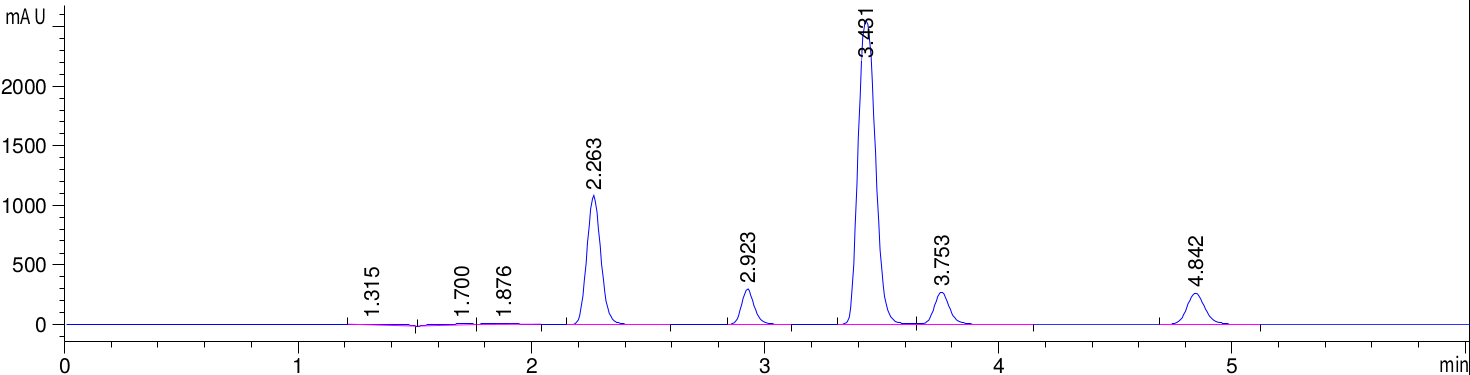
\includegraphics[scale=0.3, center]{images/Chromatogramm_PharmaMix.png} 
      \caption[Chromatogramm des Pharmazeutika-Mix, Quelle: Autor]{Chromatogramm des \SI[mode=text]{50}{ppm} Pharmazeutika-Mix.}
      \label{fig:Pharmamix}
    \end{figure}
    
    \begin{table}[H]
      \centering
      \caption[Auflistung der chromatographischen Parameter beim Pharmazeutika-Mix, Quelle: Autor]{Auflistung der chromatographischen Parameter beim Pharmazeutika-Mix ($t_0 = \SI[mode=text]{1.452}{\minute}$, $L = \SI[mode=text]{150000}{\micro\meter}$).}
      
      \label{tab:Chromatographische Parameter}
      \begin{tabular}{@{}l|lllllp{4.5cm}l@{}}
        \toprule
          Peak Nr. & Analyt & $t_R$ in \si{\minute} & $w$ in \si{\minute} & $N$ & $H$ in \si{\micro\meter} \\ \midrule
          1 & Carbamazepin & 2.263 & 0.0646 & 19635 & 7.639 \\
          2 & Estradiol & 2.923 & 0.0580 & 40637 & 3.691 \\
          3 & Naproxen & 3.431 & 0.0840 & 26693 & 5.619 \\ 
          4 & Estron & 3.753 & 0.0680 & 48737 & 3.078 \\ 
          5 & Ibuprofen & 4.842 & 0.0817 & 56199 & 2.669 \\
            &  &  &  &  &  \\ 
          Auflösung & $t_{R}'$ in \si{\minute} & $t_{R}''$ in \si{\minute} & $w'$ in \si{\minute} & $w''$ in \si{\minute} &  R \\ \midrule
          Peak 1 / Peak 2 & 2.263 & 2.923 & 0.0646 & 0.0580 & 10.8 \\
          Peak 2 / Peak 3 & 2.923 & 3.431 & 0.0580 & 0.0840 & 7.15 \\
          Peak 3 / Peak 4 & 3.431 & 3.753 & 0.0840 & 0.0680 & 4.24 \\
          Peak 4 / Peak 5 & 3.753 & 4.842 & 0.0680 & 0.0817 & 14.5 \\ \bottomrule
      \end{tabular}
    \end{table}
    
  \subsection{Quantitative Bestimmung von Wasserrückständen nach der Methode des externen Standards} 
    
    In Tabelle \ref{tab:MessungKalibrierstandardCarbamazepin} werden die Messwerte der Kalibrierstandards von Carbamazepin aufgelistet, wobei die Peakfläche als Quantifizierungsparameter verwendet wird. In Abbildung \ref{fig:KalibriergeradeCarbamazepin} ist die aus diesen Daten berechnete Kalibriergerade dargestellt. 
    
      \begin{table}[H]
        \centering
        \caption[Messung der Kalibrierstandardlösungen von Carbamazepin, Quelle: Autor]{Messung der Kalibrierstandardlösungen von Carbamazepin.}
      
        \label{tab:MessungKalibrierstandardCarbamazepin}
        \begin{tabular}{@{}lllp{4.5cm}l@{}}
          \toprule
          $c_{Std.}$ in \si{ppm} & $t_R$ in \si{\minute} & Peakfläche $A$ in \si{mAu\cdot s} \\ \midrule
            10 & 2.254 & 852.56478 \\
            10 & 2.244 & 851.82837 \\
            10 & 2.243 & 897.52515 \\
            20 & 2.252 & 1802.90051 \\
            20 & 2.247 & 1759.14392 \\
            20 & 2.245 & 1758.21021 \\
            30 & 2.246 & 2712.86621 \\
            30 & 2.250 & 2665.03857 \\
            30 & 2.251 & 2705.32861 \\
            40 & 2.243 & 3515.59009 \\
            40 & 2.252 & 3511.57788 \\
            40 & 2.241 & 3557.95532 \\
            50 & 2.245 & 4439.73486 \\
            50 & 2.247 & 4444.31152 \\
            50 & 2.239 & 4442.79785 \\ \bottomrule
        \end{tabular}
      \end{table} 
    
      \begin{figure}[H]
        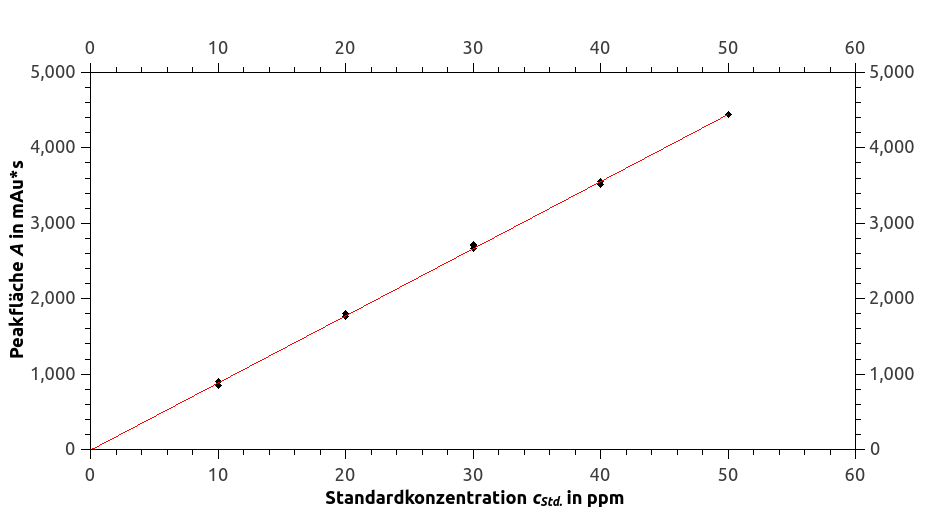
\includegraphics[scale=0.4, center]{images/Kalibriergerade.png} 
        \caption[Kalibriergerade für Carbamazepin, Quelle: Autor]{Kalibriergerade für Carbamazepin in der Form $y = a + bx$.}
        \label{fig:KalibriergeradeCarbamazepin}
      \end{figure}
    \noindent Folgende Parameter der Kalibriergeraden wurden bestimmt: Steigung $b = \SI[mode=text]{89.05}{mAus\per ppm}$, Ordinatenabschnitt $a = \SI[mode=text]{-10.314}{mAus}$, Bestimmtheitsmaß $R^2 = 0.9995$, Reststandardabweichung $s_y = 28.81$ und Freiheitsgrade $df = 13$. Die Reststandardabweichung $s_y$ wurde mit 
    
      \begin{equation}
        s_y = \sqrt{\frac{\sum_{i=1}^N \left(y_i - \overline{y_i}\right)^2}{N-2}}
      \end{equation}
    berechnet (gemessene Werte der Standards $y_i$, Erwartungswert $\overline{y_i}$, Anzahl der Messwerte $N$). Die Ergebnisse der Probemessung und das dazugehörige Chromatogramm werden in Tabelle \ref{tab:ErgebnisseProbemessung} bzw. in Abbildung \ref{fig:ChromatogrammProbemessung} festgehalten. Die Konzentration der Probe, $c_{Probe}$ wurde durch umstellen der Kalibriergeraden auf $x$ berechnet:
    
      \begin{equation}
        c_{Probe} = \frac{y - a}{b}
      \end{equation}.
    Zur Bestimmung der Peaksymmetrie wurden die Chromatogramme der Probenmessungen ausgedruckt, mit Bleistift eine Referenzlinie durch den Peak gezeichnet und in ca. \SI[mode=text]{10}{\percent} der Peakhöhe mit einem Geodreieck die Parameter $A$ und $B$ bestimmt (siehe Kapitel \ref{sec:ChromatographischeParameter})\footnote{Bei der Abgabe in gedruckter Form werden die auf diese Weise ausgewerteten Chromatogramme angehängt.}. 
    
      \begin{table}[H]
        \centering
        \caption[Ergebnisse der Probemessung, Quelle: Autor]{Ergebnisse der Probemessung (Probe Nr. 6, Substanz: Carbamazepin, $t_0 = \SI[mode=text]{1.452}{\minute}$.}
      
        \label{tab:ErgebnisseProbemessung}
        \begin{tabular}{@{}l|llllllp{4.5cm}l@{}}
          \toprule
          Nr. & $t_R$ in \si{\minute} & Peakfläche $A$ in \si{mAu\cdot s} & $c_{Probe}$ in \si{ppm} & $w$ in \si{\minute} & Kapazitätsf. $k$ & Peaksymmetrie $T$ \\ \midrule
            1 & 2.266 & 3715.58032 & 41.84 & 0.0592 & 1.561 & 1.3 \\
            2 & 2.265 & 3713.09033 & 41.81 & 0.0590 & 1.560 & 1.1 \\
            3 & 2.259 & 3880.03760 & 43.69 & 0.0608 & 1.556 & 1.4 \\ \midrule
            $\overline{x_i}$ & 2.263 & 3769.56942 & 42.45 & 0.0597 & 1.559 & 1.3 \\ \bottomrule
        \end{tabular}
      \end{table} 
    
    \pagebreak
     
    \noindent Die Standardabweichung $s_x$ berechnet kann mit
    
      \begin{equation}
        \begin{split}
          s_x &= \frac{s_y}{b} \sqrt{\frac{1}{n} + \frac{1}{m} + \frac{\left(y_0 - \overline{y}\right)^2}{b^2 \sum_{i=1}^{n} \left(x_i - \overline{x}\right)^2}} \\
              &= \frac{28.81}{89.05} \sqrt{\frac{1}{15} + \frac{1}{3} + \frac{\left(3769.57 - 2661.16\right)^2}{89.05^2 \cdot 1000}} = \SI[mode=text]{0.241}{ppm}
        \end{split}
      \end{equation}
    berechnet werden (Anzahl an Kalibriermessungen $n$, Anzahl an Probemessungen $m$, Reststandardabweichung $s_y$, Steigung $b$, Mittelwert der Kalibriersignale $\overline{y}$, Mittelwert des Probensignals $y_0$, Konzentration des jeweiligen Standards $x_i$). Der Vertrauensbereich $T_x$ ($\alpha = 0.05$ und $t = 2.160$ für $df = 13$) kann mit 
    
      \begin{equation}
        T_x = s_x t = \SI[mode=text]{0.521}{ppm}
      \end{equation}  
    berechnet werden. Damit ist die Konzentration an Carbamazepin in der Probelösung: 
    
    \noindent $c_{Probe} = \SI[mode=text, multi-part-units = brackets, separate-uncertainty]{42.5(5)}{ppm} \left(N = 15, m = 3, s_x = \SI[mode=text]{0.241}{ppm}, \alpha = 0.05\right)$.
      
      \begin{figure}[H]
        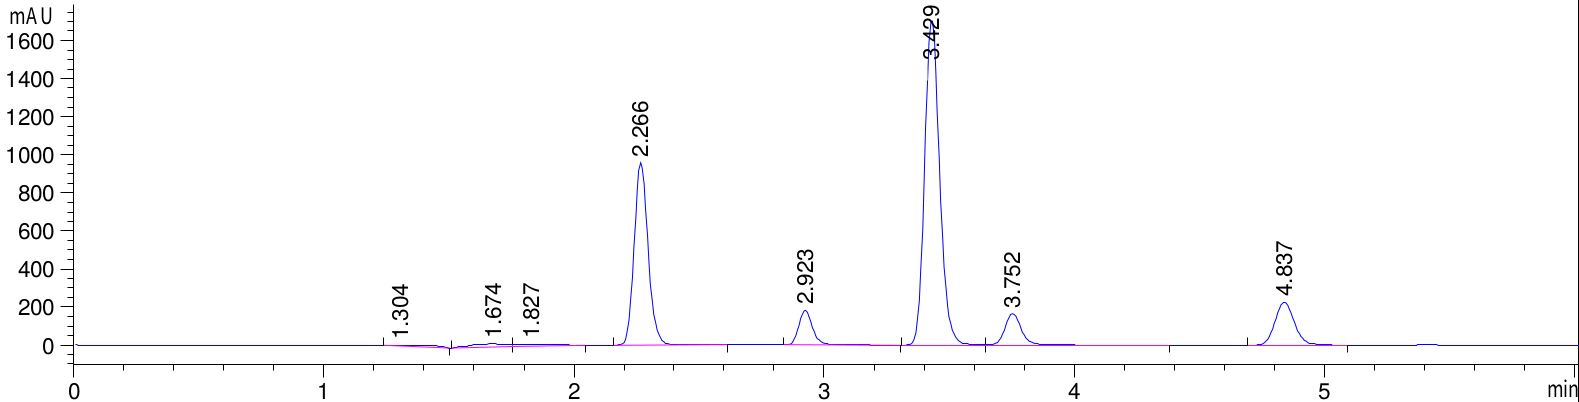
\includegraphics[scale=0.28, center]{images/Probemessung1.png} 
        \caption[Chromatogramm von Probemessung Nr. 1, Quelle: Autor]{Chromatogramm von Probemessung Nr. 1.}
        \label{fig:ChromatogrammProbemessung}
      \end{figure}
    
    
   
    
      